\documentclass[tikz,border=2pt]{standalone}
\usepackage{amsmath,amssymb}
\usepackage{tikz}
\usetikzlibrary{arrows.meta}

\begin{document}
% Eight observations on a number line and their sample mean 5.0: the point where the data
% balance (deviations to the left and right cancel).
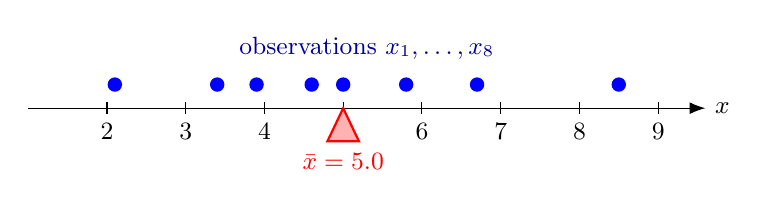
\begin{tikzpicture}[every node/.style={font=\small}, >={Latex[length=2mm]}]
	\draw[->] (1,0) -- (9.6,0) node[right] {$x$};
	\foreach \x in {2,3,...,9} {\draw (\x,0.08) -- (\x,-0.08); \node[below=2pt, font=\small] at (\x,0) {\x};}
	\foreach \x in {2.1,3.4,3.9,4.6,5.0,5.8,6.7,8.5} {\fill[blue] (\x,0.3) circle (2.6pt);}
	\draw[red, thick, fill=red!30] (5,0) -- (4.8,-0.42) -- (5.2,-0.42) -- cycle;
	\node[red, anchor=north] at (5,-0.45) {$\bar x=5.0$};
	\node[blue!60!black, anchor=south] at (5.3,0.5) {observations $x_1,\dots,x_8$};
	
\end{tikzpicture}
\end{document}
